
\chapter{Delineamento Metodológico}\label{delineamento}

Nesta pesquisa foi realizado um experimento onde os dados coletados permitam comparar a performance do binário gerado por dois compiladores na plataforma WebAssembly, com isso, trata-se de uma pesquisa experimental e quantitativa \cite{metodologia}. Além disso, quanto ao seu objetivo, trata-se de uma pesquisa descritiva, pois tem o objetivo de obter dados de um experimento e descreve-los \cite{gil}.

\section{Descrição do experimento}\label{descricao_experimento}

Para realizar o experimento, foi criado \textit{scripts} escritos nas linguagens bash, Python e JS que são responsáveis por executar o experimento de forma automática. Dessa forma, o experimento pôde avançar rápido com pouca intervenção humana que poderia ocasionar erros.

\section{Captura de métricas utilizadas}\label{manipulacoes}

Nessa seção será explicado como é capturado as métricas utilizadas na pesquisa, além de explicar as decisões tomadas sobre como realizar a captura.

\begin{quadro}
\caption{Arquivo \code{cheerp\_capture\_time.js} adicionado ao código emitido pelo Cheerp}
\begin{lstlisting}
var polybench_time = null;
var initial_memory = null;
var memory_used = null;
var _log = console.log;
function capture_time(time) {
    polybench_time = parseFloat(time);
    console.log = _log;
}
console.log = capture_time;
\end{lstlisting}
\label{cheerp_capture_time}
\end{quadro}


A função \code{\_\_start} citada é responsável por iniciar a execução do algoritmo. Portanto, a primeira instrução captura a quantidade de memória antes da execução algoritmo, enquanto a segunda instrução captura a memória final, após a execução. Além disso, é também adiciona a instrução \code{return} que retorna para o usuário uma estrutura com as três métricas capturadas, permitindo que elas possam ser salvas em disco.

\section{Processo de execução no navegador}\label{execucao}

Nesta seção será descrito o que ocorre na etapa onde um navegador é aberto e executado um binário WebAssembly, essa etapa é repetida para cada algoritmo e para cada navegador. Antes dos navegadores serem abertos pelo executável do apêndice \ref{run_script}, é executado um programa na linguagem de programação Python pelo próprio \textit{script} através do comando \code{python3 -m http.server}. 

\begin{figure}[h]
    \centering
    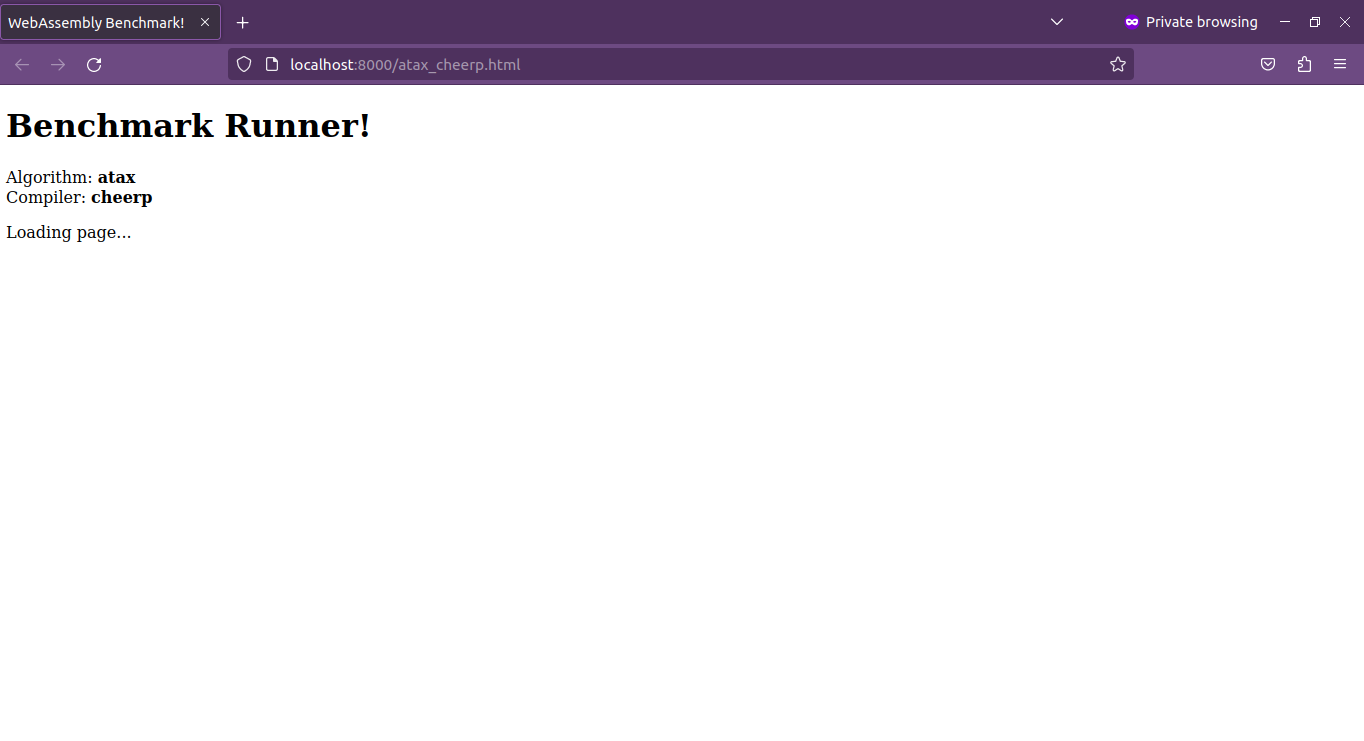
\includegraphics[scale=0.3]{images/html_firefox.png}
    \caption{Arquivo HTML aberto no navegador Firefox para o algoritmo \code{atax}}
    \label{fig:html}
\end{figure}

Na figura é apresentado o texto \textit{Loading page...}, ele permanece por um segundo para certificar-se que o navegador foi inicializado corretamente. Esse texto é alterado automaticamente conforme o experimento progride para informar o pesquisador o estágio que está sendo realizado.
 
\section{Descrição do ambiente}

Foi rodado na máquina do laboratório

